\documentclass[11pt,letterpaper]{article}
\usepackage[lmargin=1in,rmargin=1in,tmargin=1in,bmargin=1in]{geometry}
\usepackage{homework}

% -------------------
% Content
% -------------------
\begin{document}
\homework{Solutions --- Caleb McWhorter}

% Problem 1
\problem{10} Let $f: A \to \mathbb{R}$ be defined by $f(x):= x^3 - 9x^2 + 23x - 12$, where $A= \{ 1, 3, 6 \}$. Let $g: B \to \mathbb{R}$ be defined by $g(x)= x^2 - 4x + 6$, where 
	\[
	B= \{ x \in \mathbb{N} \;|\; x \text{ divides }6 \} \setminus \{x \colon x \text{ is an even prime number} \}
	\]
Prove that $f= g$. \pspace

\sol To prove two functions are equal, we need to show that\dots

\textbullet\ {\itshape The functions have the same domain:}

The domain for $f$ is $A$ and the domain for $g$ is $B$. So we need to show that $A= B$. Observe that\dots
	\[
	\begin{aligned}
	B&= \{ x \in \mathbb{N} \;|\; x \text{ divides }6 \} \setminus \{x \colon x \text{ is an even prime number} \} \\
	&= \{ 1, 2, 3, 6 \} \setminus \{ 2 \} \\
	&= \{ 1, 3, 6 \}
	\end{aligned}
	\]
But then it is clear that $A= B$. \pspace

\textbullet {\itshape The functions have the same codomain.} \pspace

This is immediate because the codomain of $f$ and $g$ are the same---namely $\mathbb{R}$. \pspace

\textbullet {\itshape The functions are equal everywhere on their common domain.} \pspace

The domain for both functions is $\{ 1, 3, 6 \}$. Observe\dots
	\[
	\begin{aligned}
	f(1)&= 1^3 - 9(1^2) + 23(1) - 12= 1 - 9 + 23 - 12= 3 \\
	g(1)&= 1^2 - 4(1) + 6= 1 - 4 + 6= 3 \\
	\\
	f(3)&= 3^3 - 9(3^2) + 23(3) - 12= 27 - 81 + 69 - 12= 3 \\
	g(3)&= 3^2 - 4(3) + 6= 9 - 12 + 6= 3 \\
	\\
	f(6)&= 6^3 - 9(6^2) + 23(6) - 12= 216 - 324 + 138 - 12= 18 \\
	g(6)&= 6^2 - 4(6) + 6= 36 - 24 + 6= 18
	\end{aligned}
	\] \pspace
Therefore, we know that $f= g$. 



\newpage



% Problem 2
\problem{10} Recall the absolute value function, $f(x)= |x|$, is given by
	\[
	|x|= 
	\begin{cases}
	x, & x \geq 0 \\
	-x, & x < 0 
	\end{cases}
	\]
Considering $f: \mathbb{R} \to \mathbb{R}$, determine the following sets:
	\begin{enumerate}[(a)]
	\item $f((-2, 1])$
	\item $f(\mathbb{Z})$
	\item $f^{-1}((-2,1])$
	\item $f^{-1}(\{-5\})$
	\item $f^{-1}(\mathbb{Z})$
	\end{enumerate} \pspace

\sol Let $f(x)= |x|$. If $S$ is a set of real numbers, let $\pm |S|:= \{ \pm |s| \colon s \in S \}$. Observe that because $f(P)= \{ f(p) \colon p \in P \}$, if $P$ is a set of nonnegative real numbers, then $f(P)= P$. Moreover, because $f(N)= \{ f(n) \colon n \in N \}$, if $N$ is a set of negative real numbers, we know that $f(N)= \{ f(n) \colon n \in N \}= \{ f(|n|) \colon n \in N \}= f(|N|)= |N|$. But then given a set $S$ of real numbers, we can decompose $S= P \cup N$ into a set of nonnegative numbers, $P$, and negative numbers, $N$, respectively. But then we have $f(S)= f(P \cup N)= f(P) \cup f(N)= P \cup |N|$. \pspace

Now recall that $f^{-1}(S)$ is the preimage of $S$ under $f$, i.e. the set of $x \in \mathbb{R}$ such that $f(x) \in S$. As above, let $P$ contain only nonnegative real numbers and $N$ consists of only negative real numbers. Clearly, $f^{-1}(N)= \varnothing$ because $f(x) \geq 0$ for all $x \in \mathbb{R}$, i.e. $f(x) \notin N$ for all $x \in \mathbb{R}$. Now let $p \in P$. Clearly, $f(\pm p)= | \pm p|= p$. But then $f^{-1}(P)= \{ \pm p \colon p \in P \}$. 

\sol 
\begin{enumerate}[(a)]
\item We have\dots
	\[
	f\big( (-2, 1] \big)= f \big( (-2,0) \cup [0, 1] \big)= f\big( (-2, 0) \big) \cup f \big( [0, 1] \big)= (0, 2) \cup [0, 1]= [0, 2)
	\] \pspace

\item 
	\[
	f(\mathbb{Z})= f \left( \mathbb{Z}_{< 0} \cup \mathbb{Z}_{\geq 0} \right)=  f \left( \mathbb{Z}_{< 0} \right) \cup f \left( \mathbb{Z}_{\geq 0} \right)= |\mathbb{Z}_{< 0}| \cup \mathbb{Z}_{\geq 0}= \mathbb{Z}_{> 0} \cup \mathbb{Z}_{\geq 0}= \mathbb{Z}_{\geq 0}
	\] \pspace

\item 
	\[
	f^{-1} \big( (-2, 1] \big)= f^{-1} \big( (-2, 0) \cup [0, 1] \big)= f^{-1} \big( (-2, 0) \big) \cup f^{-1} \big( [0, 1] \big)= \varnothing \cup \{ \pm r \colon r \in [0, 1] \}= [-1, 1]
	\] \pspace

\item 
	\[
	f^{-1} \big( \{ -5 \} \big)= \varnothing
	\] \pspace

\item 
	\[
	f^{-1} (\mathbb{Z})= f^{-1} \left( \mathbb{Z}_{< 0} \cup \mathbb{Z}_{\geq 0} \right) = f^{-1} \left( \mathbb{Z}_{< 0} \right) \cup f^{-1} \left( \mathbb{Z}_{\geq 0} \right)= \varnothing \cup \{ \pm z \colon z \in \mathbb{Z}_{\geq 0} \}= \mathbb{Z}
	\]
\end{enumerate}



\newpage



% Problem 3
\problem{10} Let $f: \mathbb{Z} \to \mathbb{R}$ be given by $f(n)= 2^n$, and let $g: \mathbb{Z} \to \mathbb{R}$ be given by $g(n)= 100 - 3^n$. 
\begin{enumerate}[(a)]
\item Compute $f(1)$.
\item Compute $g(1)$.
\item Compute $(fg)(1)$.
\item Compute $(f \circ g)(1)$.
\item Find the rule for $(fg)(x)$.
\end{enumerate} \pspace

\sol 
\begin{enumerate}[(a)]
\item 
	\[
	f(1)= 2^1= 2
	\] \pspace

\item 
	\[
	g(1)= 100 - 3^1= 100 - 3= 97
	\] \pspace

\item 
	\[
	(fg)(1)= f(1) \cdot g(1)= 2 \cdot 97= 194
	\] \pspace

\item 
	\[
	(f \circ g)(1)= f \big( g(1) \big)= f(97)= 2^{97}= 158,\!456,\!325,\!028,\!528,\!675,\!187,\!087,\!900,\!672
	\] \pspace

\item 
	\[
	(fg)(x)= f(x) \cdot g(x)= 2^x (100 - 3^x)
	\]
\end{enumerate}



\newpage



% Problem 4
\problem{10} Recall that given a function $f: S \to S$, we say that $x \in S$ is a fixed point of $f$ if $f(x)= x$. Let $S= \mathbb{R}$ and let $f$ be the function given by $x \mapsto x^2 + 4x - 10$. Find the fixed points of $f$. How does the answer change if $S= \mathbb{N}$? \pspace

\sol We know that $f: \mathbb{R} \to \mathbb{R}$ is given by $f(x)= x^2 + 4x - 10$. If $x$ is a fixed point for $f$, then $f(x)= x$. But then\dots
	\[
	\begin{gathered}
	f(x)= x \\
	x^2 + 4x - 10= x \\
	x^2 + 3x - 10= 0 \\
	(x + 5)(x - 2)= 0 
	\end{gathered}
	\]
This implies that either $x + 5= 0$, so that $x= -5$, or $x - 2= 0$, so that $x= 2$. Observe that $f(-5)= (-5)^2 + 4(-5) - 10= 25 - 20 - 10= -5$ and $f(2)= 2^2 + 4(2) - 10= 4 + 8 - 10= 2$, which shows that $-5, 2$ are fixed points for $f(x)$. \pspace

Now consider $f(x)$ as a function $f: \mathbb{N} \to \mathbb{N}$. The solution $x= -5$ is no longer valid because $-5 \notin \mathbb{N}$. But then the only fixed point for $f(x)$ would be $x= 2$. 



\newpage



% Problem 5
\problem{10} Recall that the image of a function $f: S \to S$ (also called the range) is the set $\im f= \{ f(s) \colon s \in S \}$. Consider the function $f: \mathbb{R} \to \mathbb{R}$ defined by $f(x)= \dfrac{1}{1 + x^2}$. 
\begin{enumerate}[(a)]
\item Determine the error in the following `proof' that $\im f= \mathbb{R}$: \pspace

{\itshape We need prove that $\im f \subseteq \mathbb{R}$ and $\mathbb{R} \subseteq \im f$. Clearly, $f(x) \in \mathbb{R}$ so that $\im f \subseteq \mathbb{R}$. Now let $y \in \mathbb{R}$. Define $x:= \sqrt{\dfrac{1 - y}{y}}$. Then
	\[
	f(x)= \dfrac{1}{1 + x^2}= \dfrac{1}{1 + \dfrac{1 - y}{y}}= \dfrac{1}{\dfrac{y + 1 - y}{y}}= \dfrac{1}{1/y}= y.
	\]
But then $x \in \mathbb{R}$ and $f(x)= y$. Therefore, $\mathbb{R} \subseteq \im f$. Because $\im f \subseteq \mathbb{R}$ and $\mathbb{R} \subseteq \im f$, $\im f = \mathbb{R}$.}

\item Determine $\im f$ and prove that your answer is correct. 
\end{enumerate} \pspace

\sol 
\begin{enumerate}[(a)]
\item The first sentence is correct---two sets are equal if and only if they are subsets of each other. The second sentence is also true---the outputs of $f(x)$ are real numbers (because the inputs are real) so that $\im f \subseteq \mathbb{R}$. The third sentence is fine, one can declare $y$ to be some real number. However, the next sentence has an error. We took $y \in \mathbb{R}$ to be \textit{any} real number and defined a (hopefully) real number $x$. But the definition of $x$ should then work for any $y$-value. If $y= -1$, then $x= \sqrt{\dfrac{1 - (-1)}{-1}}= \sqrt{\dfrac{2}{-1}}= \sqrt{-2}$ is not a real number. The next sentence is true, if $x$ is a real number (so that it is in the domain of $f$), then the evaluation of $f(x)= y$ is correct so that $y \in \mathbb{R}$ is in the range of $f(x)$. Therefore, the error in the proof is the fact that the defined $x$ may not be a real number. \pspace

\item Based on (a), we see that the proof fails because $x$ may not be a real number. For $x$ to be defined, we need $\frac{1 - y}{y} \geq 0$. Clearly, $y \neq 0$. Furthermore, if $y < 0$, then $-y > 0$ so that $1 - y > 1 > 0$ and then $\frac{1 - y}{y} < 0$ (because $y < 0$). Finally, suppose $y \geq 0$. Then $\frac{1 - y}{y} \geq 0$ implies that $1 - y \geq 0$ so that $1 \geq y$. As $y > 0$, this implies $0 < y \leq 1$. We would then conjecture that $\im f= (0, 1]$, which we shall prove. In fact, the proof above works with little modification! \pspace

We need prove that $\im f \subseteq (0, 1]$ and $(0, 1] \subseteq \im f$. Because $x \in \mathbb{R}$, we know that $x^2 \geq 0$. But then $1 + x^2 \geq 1$, so that $f(x)= \frac{1}{1 + x^2} \leq 1$. Finally, because $1 + x^2 > 0$, we know that $f(x)= \frac{1}{1 + x^2} > 0$. Therefore, $0 < f(x) \leq 1$. This proves that $\im f \subseteq (0, 1]$. 

Now let $y \in (0, 1]$. Then $1 \geq y$ so that $1 - y \geq 0$. But because $y > 0$, this implies that $\frac{1 - y}{y} \geq 0$. Now because $\frac{1 - y}{y} \geq 0$, we can define $x:= \sqrt{\dfrac{1 - y}{y}}$. Then
	\[
	f(x)= \dfrac{1}{1 + x^2}= \dfrac{1}{1 + \dfrac{1 - y}{y}}= \dfrac{1}{\dfrac{y + 1 - y}{y}}= \dfrac{1}{1/y}= y.
	\]
But then $x \in \mathbb{R}$ and $f(x)= y$. Therefore, $(0, 1] \subseteq \im f$. Because $\im f \subseteq (0, 1]$ and $(0, 1] \subseteq \im f$, $\im f = (0, 1]$. \pspace

We might have predicted this to be the image of $\mathbb{R}$ under $f$ by examining the graph of $f(x)$:
	\[
	\fbox{
	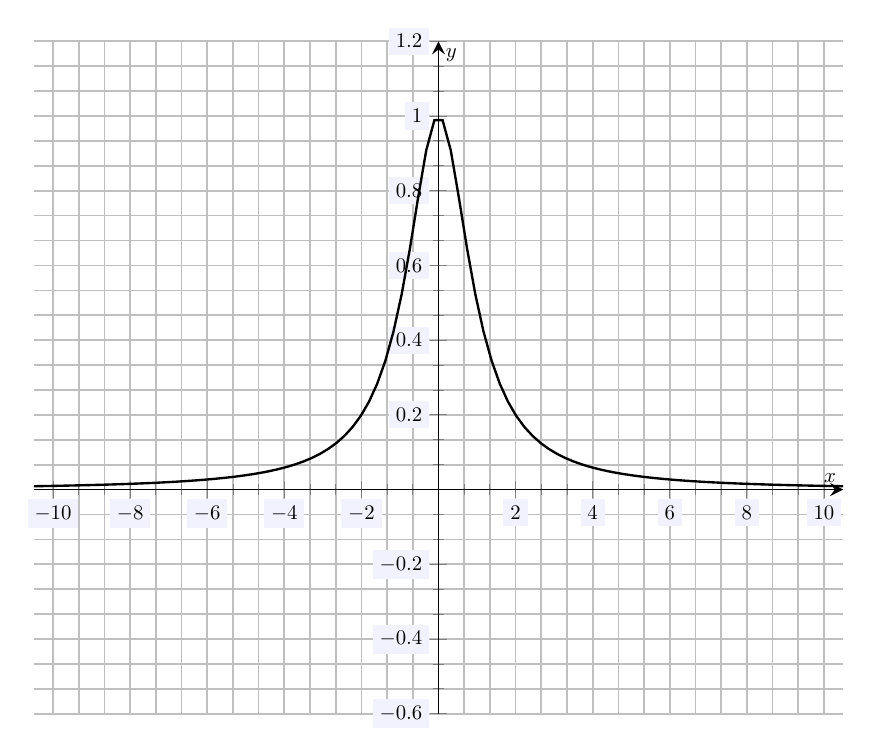
\begin{tikzpicture}[scale=1.5,every node/.style={scale=0.5}]
	\begin{axis}[
	grid=both,
	axis lines=middle,
	ticklabel style={fill=blue!5!white},
	xmin= -10.5, xmax=10.5,
	ymin= -0.6, ymax=1.2,
	xtick={-10,-8,-6,-4,-2,0,2,4,6,8,10},
	ytick={-0.6,-0.4,...,1.2},
	minor x tick num= 2,
	minor y tick num= 2,
	xlabel=\(x\),ylabel=\(y\),
	]
	\addplot[line width= 0.02cm,samples=100,domain= -10.5:10.5] ({x},{1/(1 + x^2)}); 

	\end{axis}
	\end{tikzpicture}
	}
	\] 
\end{enumerate}


\end{document}